\begin{enumerate}
\item From a point $Q$, $13 \text{ cm}$ away from the centre of a circle, the length of tangent $PQ$ to the circle is $12 \text{ cm}$. The radius of circle \brak{\text{in $cm$}}
\begin{enumerate}
\item $25$ 
\item $\sqrt{313}$ 
\item $5$ 
\item $1$ 
\end{enumerate}
%circles
\item In Figure $1$, $AP$, $AQ$ and $BC$ are tangents to the circle. If $AB = 5 \text{cm}$, $AC = 6 \text{ cm}$ and $BC = 4 \text{ cm}$, then the length of $AP$ \brak{\text{in $cm$}} is
\begin{figure} [h]
\centering
\begin{tikzpicture}[scale=1.2]

% Circle
\draw (0,0) circle (1cm);

% Points
\coordinate (A) at (0,3);
\coordinate (B) at (-0.7, 1);
\coordinate (C) at (0.7, 1);
\coordinate (P) at (-0.95, 0.3);
\coordinate (Q) at (0.95, 0.3);

% Tangents and Lines
\draw (A) -- (B) node[midway, left] {};
\draw (A) -- (C) node[midway, right] {};
\draw (B) -- (C) node[midway, below] {};
\draw (B) -- (P);
\draw (C) -- (Q);

% Arrows
\draw[->] (P) -- ($(B)!2cm!(P)$);
\draw[->] (Q) -- ($(C)!2cm!(Q)$);

% Perpendicular lines
\draw ($(P)!0.1cm!90:(B)$) -- ($(P)!0.1cm!-90:(B)$);
\draw ($(Q)!0.1cm!90:(C)$) -- ($(Q)!0.1cm!-90:(C)$);

% Labeling points
\node at (A) [above] {A};
\node at (B) [left] {B};
\node at (C) [right] {C};
\node at (P) [left] {P};
\node at (Q) [right] {Q};
\end{tikzpicture}
\end{figure}
\begin{center}
$\text{Figure } 1$
\end{center}
\begin{enumerate}
\item $7.5$ 
\item $15$ 
\item $10$ 
\item $9$ 
\end{enumerate}
%circles
\item The circumference of a circle is $22 \text{ cm}$. The area of its quadrant \brak{\text{in $cm^2$}}
\begin{enumerate}
\item $\dfrac{77}{2}$ 
\item $\dfrac{77}{4}$ 
\item $\dfrac{77}{8}$ 
\item $\dfrac{77}{16}$ 
\end{enumerate}
\item In Figure $2$, a right triangle $ABC$, circumscribe a circle of radius $r$. If $AB$ and $BC$ are of lengths $8 \text{ cm}$ and $6 \text{ cm}$ respectively, find the value of $r$.
\begin{figure}[ht]
\centering
\begin{tikzpicture}[scale=0.6]
    % Triangle ABC
    \coordinate[label=above:$A$] (A) at (0,8);
    \coordinate[label=below left:$B$] (B) at (0,0);
    \coordinate[label=below:$C$] (C) at (6,0);
    \draw (A) -- (B) -- (C) -- cycle;
    
    % Point (18/5, 16/5)
    \coordinate[label=above:$ $] (P) at (3.6,3.2);
    \fill (P) circle (0pt);
    
    % Line and length r
    \draw[thick] (2,2) -- (3.6,3.2);
    \node[label=below left:$O$,circle,fill,inner sep=1.5pt] (O) at (2,2) {};
    \node[label=above:$r$] at (2.8,2.6) {};
    \draw (O) circle (2cm);
    % Right angle at B
    \draw pic["$ $", draw=black, angle radius=0.4cm, angle eccentricity=1.5] {right angle = C--B--A};
\end{tikzpicture}
\end{figure}
\begin{center}
$\text{Figure } 2$
\end{center}
\item In Figure $3$, $PQ$ and $PR$ are tangents to a circle with centre $A$. If $\angle QPA = 27\degree$, then $\angle QAR$ equals
\begin{figure}[ht]
\centering
\begin{tikzpicture}[scale=1.3]
  % Define points
  \coordinate (A) at (0,0);
  \coordinate (Q) at (0.45,0.9); % This point is 60 degrees above the horizontal.
  \coordinate (P) at (2,0);     % Chosen arbitrarily, adjust as needed.
  \coordinate (R) at (0.45,-0.9); % Midpoint of AP
  
  % Draw circle with center A through point Q
  \draw (A) circle (1cm);
  
  % Draw triangle APQ
  \draw (A) -- (P) -- (Q) -- cycle;
  \draw (A) -- (P) -- (R) -- cycle;
  \draw (0.45,0.9) -- (-0.415,1.402);
  \draw (0.45,-0.9) -- (-0.415,-1.402);
  
  % Label points
  \node at (A) [left] {A};
  \node at (P) [right] {P};
  \node at (Q) [above] {Q};
  \node at (R) [below] {R};
  \fill (0,0) circle (0.75pt);

  % Draw the angle arc % Draw the angle with label
  \pic [draw, "$ $", angle eccentricity = 1, angle radius=0.5cm] {angle = Q--P--A};


\end{tikzpicture}
\end{figure}
\begin{center}
$\text{Figure } 3$
\end{center}
\begin{enumerate}
\item $63\degree$ 
\item $153\degree$ 
\item $126\degree$ 
\item $117\degree$ 
\end{enumerate}
\item In Figure $4$, $AB$ and $AC$ are tangents to a circle with centre $O$ and radius $8\text{ cm}$. If $OA = 17\text{ cm}$, then the length of $AC \brak{\text { in cm}}$  is
\begin{figure}[ht]
\centering
\begin{tikzpicture}[scale=1.3]
  % Define points
  \coordinate (O) at (0,0);
  \coordinate (B) at (0.45,0.9); % This point is 60 degrees above the horizontal.
  \coordinate (A) at (2,0);     % Chosen arbitrarily, adjust as needed.
  \coordinate (C) at (0.45,-0.9); % Midpoint of AP
  
  % Draw circle with center A through point Q
  \draw (O) circle (1cm);
  
  % Draw triangle APQ
  \draw (O) -- (A) -- (B) -- cycle;
  \draw (A) -- (C);
  \draw (0.45,0.9) -- (-0.415,1.402);
  \draw (0.45,-0.9) -- (-0.415,-1.402);
  \draw ($(C)!0.05cm!90:(A)$) -- ($(C)!0.05cm!-90:(A)$);
  
  % Label points
  \node at (O) [left] {O};
  \node at (A) [right] {A};
  \node at (B) [above] {B};
  \node at (C) [below] {C};
  \fill (0,0) circle (0.75pt);

\end{tikzpicture}
\end{figure}
\begin{center}
$\text{Figure } 4$
\end{center}
\begin{enumerate}
\item $\sqrt {353}$ 
\item $15$ 
\item $9$ 
\item $25$ 
\end{enumerate}
\item In Figure $5$, three sectors of a circle of radius $7\text{ cm}$, making angles of $60\degree$, $80\degree$, $40\degree$ at the centre are shaded. The area of the shaded region $\brak{in\text{ cm}^2}$ is $\brak{\text{Using } \pi = \frac{22}{7}}$
\begin{figure}[ht]
\centering
\begin{tikzpicture}[scale = 1.4, rotate=10]
  % Define the radius of the circle
  \def\radius{1cm}
  
  % Draw the circle
  \draw (0,0) circle (1cm);
  
  % Define points for the angles
  \coordinate (O) at (0,0);
  \coordinate (A) at (1,0);
  \coordinate (C) at (80:1);
  \coordinate (D) at (160:1);
  \coordinate (E) at (200:1);
  \coordinate (F) at (240:1);
  \coordinate (B) at (300:1);

  % Draw the angle arc % Draw the angle with label
  \pic [draw, "$60^O$", angle eccentricity=1.75, angle radius=0.4cm] {angle = B--O--A};
  \pic [draw, "$80^O$", angle eccentricity=1.75, angle radius=0.4cm] {angle = C--O--D};
  \pic [draw, "$40^O$", angle eccentricity=1.75, angle radius=0.4cm] {angle = E--O--F};
  
  % Draw the sectors and lines
  \draw (O) -- (A) (O) -- (B) (O) -- (C);
  \draw (O) -- (D) (O) -- (E) (O) -- (F);

  \fill[pattern=north east lines] (0,0) circle (1cm);

  % Draw the quadrants
  \draw[fill=white] (O) -- (A) arc [start angle=0, end angle=80, radius=1] -- cycle;
  \draw[fill=white] (O) -- (D) arc [start angle=160, end angle=200, radius=1] -- cycle;
  \draw[fill=white] (O) -- (F) arc [start angle=240, end angle=300, radius=1] -- cycle;
  
  % Label the center
  \node at (O) [above right] {O};

\end{tikzpicture}
\end{figure}
\begin{center}
$\text{Figure } 5$
\end{center}
\begin{enumerate}
\item $77$ 
\item $154$ 
\item $44$ 
\item $22$ 
\end{enumerate}
\item In Figure $6$, the sides $AB$, $BC$ and $CA$ of a triangle $ABC$, touch a circle at $P$, $Q$ and $R$ respectively. If $PA = 4\text{ cm}$, $BP = 3\text{ cm}$ and $AC = 11\text{ cm}$, then the length of $BC$ \brak{\text{in $cm$}} is
\begin{figure}[ht]
\centering
\begin{tikzpicture}[scale=0.3]
  % Define coordinates for the vertices of the triangle
  \coordinate[label=left:$B$] (B) at (0,0);
  \coordinate[label=right:$C$] (C) at (10,0);
  \coordinate[label=above:$A$] (A) at (5,8.6603);

  % Draw the triangle
  \draw (A) -- (B) -- (C) -- cycle;

 % Draw the circle with centre (0.5,0.28868) and radius 0.28868
    \draw (5,2.8868) circle (2.8868);

  % Label the incenter. Adjust the label position as needed
  \coordinate[label=left:$P$] (P) at (2.5,4.33015);
  \coordinate[label=above:$Q$] (Q) at (5,0);
  \coordinate[label=right:$R$] (R) at (7.5,4.33015);
  % Drawing perpendicular lines
  \draw ($(Q)!0.1cm!90:(B)$) -- ($(Q)!0.1cm!-90:(B)$);
  \draw ($(R)!0.1cm!90:(C)$) -- ($(R)!0.1cm!-90:(C)$);
  \draw ($(P)!0.1cm!90:(B)$) -- ($(P)!0.1cm!-90:(B)$);

\end{tikzpicture}
\end{figure}
\begin{center}
$\text{Figure } 6$
\end{center}
\begin{enumerate}
\item $11$ 
\item $10$ 
\item $14$ 
\item $15$ 
\end{enumerate}
%circles
\item In Figure $7$, a circle touches the side $DF$ of $\triangle EDF$ at $H$ and touches $ED$ and $EF$ produced at $K$ and $M$ respectively. If $EK = 9\text{ cm}$, then the perimeter of $\triangle EDF$ \brak{\text{in $cm$}} is
\begin{figure}[ht]
\centering
\begin{tikzpicture}[scale=0.65]

% Circle
\draw (1,-1.732) circle (1.73234cm);

% Points
\coordinate (D) at (0,0);
\coordinate (E) at (1, 1.732);
\coordinate (F) at (2, 0);
\coordinate (H) at (1, 0);
\coordinate (K) at (-0.475, -0.8);
\coordinate (M) at (2.475, -0.8);

% Tangents and Lines
\draw (D) -- (E) node[midway, left] {};
\draw (E) -- (F) node[midway, right] {};
\draw (F) -- (D) node[midway, below] {};
\draw (D) -- (K);
\draw (F) -- (M);

% Arrows
\draw[-] (D) -- ($(D)!2.5cm!(K)$);
\draw[-] (F) -- ($(F)!2.5cm!(M)$);

% Perpendicular lines
\draw ($(K)!0.1cm!90:(D)$) -- ($(K)!0.1cm!-90:(D)$);
\draw ($(M)!0.1cm!90:(F)$) -- ($(M)!0.1cm!-90:(F)$);

% Labeling points
\node at (E) [above] {E};
\node at (D) [left] {D};
\node at (F) [right] {F};
\node at (H) [above] {H};
\node at (K) [left] {K};
\node at (M) [right] {M};

\end{tikzpicture}
\end{figure}
\begin{center}
$\text{Figure } 7$
\end{center}
\begin{enumerate}
\item $18$ 
\item $13.5$ 
\item $12$ 
\item $9$ 
\end{enumerate}
%circles
\item If the area of a circle is equal to sum of the areas of two circles of diameters $10 \text{ cm}$ and $24 \text{ cm}$, then the diameter of the larger circle \brak{\text{in $cm$}} is
\begin{enumerate}
\item $34$ 
\item $26$ 
\item $17$ 
\item $14$ 
\end{enumerate}
%Circles
\item Prove that the tangents drawn at the ends of a diameter of a circle are parallel. 
%circles
\item In Figure $8$, $ABCD$ is a square of side $4 \text{ cm}$. A quadrant of a circle of radius $1 \text{ cm}$ is drawn at each vertex of the square and a circle of diameter $2 \text{ cm}$ is also drawn. Find the area of the shaded region. $\brak{\text{Use } \pi = 3.14}$
\begin{figure}[ht]
\centering
\begin{tikzpicture}[scale=0.5]
    % Draw the square
    \draw[thick] (0,0) rectangle (4,4);
    
    % Draw the circle
    \draw[thick,fill=white] (2,2) circle [radius=1];
    
    % Draw the quadrants
    \draw[thick,fill=white] (0,0) -- (1,0) arc [start angle=0, end angle=90, radius=1] -- cycle;
    \draw[thick,fill=white] (4,0) -- (3,0) arc [start angle=180, end angle=90, radius=1] -- cycle;
    \draw[thick,fill=white] (4,4) -- (3,4) arc [start angle=180, end angle=270, radius=1] -- cycle;
    \draw[thick,fill=white] (0,4) -- (1,4) arc [start angle=360, end angle=270, radius=1] -- cycle;
    
    % Add the hatching pattern with controlled density
    \path[pattern=north east lines, pattern color=black] (0,0) rectangle (4,4);
    
    % Exclude the circle and quadrants from the hatching by overlaying with white fill
    \draw[fill=white] (2,2) circle [radius=1];
    \draw[fill=white] (0,0) -- (1,0) arc [start angle=0, end angle=90, radius=1] -- cycle;
    \draw[fill=white] (4,0) -- (3,0) arc [start angle=180, end angle=90, radius=1] -- cycle;
    \draw[fill=white] (4,4) -- (3,4) arc [start angle=180, end angle=270, radius=1] -- cycle;
    \draw[fill=white] (0,4) -- (1,4) arc [start angle=360, end angle=270, radius=1] -- cycle;
    \node at (0,0) [below left] {A};
    \node at (4,0) [below right] {B};
    \node at (4,4) [above right] {C};
    \node at (0,4) [above left] {D};
\end{tikzpicture}
\end{figure}
\begin{center}
$\text{Figure } 8$
\end{center}
%Circles
\item From a rectangular sheet of paper $ABCD$ with $AB = 40 \text{ cm}$ and $AD = 28 \text{ cm}$, a semi-circular portion with $BC$ as diameter is cut off. Find the area of the remaining paper. $\brak{\text{Use } \pi = \frac{22}{7}}$ 
%Circles
\item In Figure $9$, a circle is inscribed in a triangle $PQR$ with $PQ = 10 \text{ cm}$, $QR = 8 \text{ cm}$ and $PR = 12 \text{ cm}$. Find the lengths of $QM$, $RN$ and $PL$.
\begin{figure}[ht]
\centering
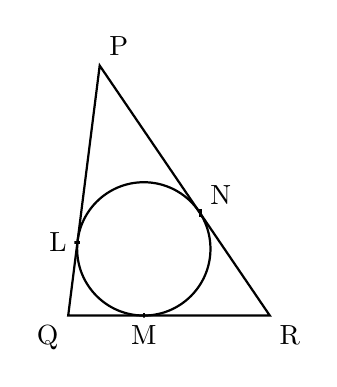
\begin{tikzpicture}[scale=0.32]

% Define points
\coordinate (P) at (1.25,9.92);
\coordinate (Q) at (0,0);
\coordinate (R) at (8,0);
\coordinate (N) at (5.25,4);
\coordinate (L) at (0.33,2.9);
\coordinate (M) at (3,0);

% Draw triangle and lines
\draw[thick] (P) -- (Q) -- (R) -- cycle;
\draw[thick] (5.25,4) -- ++(0,-0.08) -- ++(0,0.3); % Perpendicular line at N
\draw[thick] (0.33,2.9) -- ++(-0.08,0) -- ++(0.2,0); % Horizontal line at (0.33,2.9)
\draw[thick] (3,0) -- ++(0,-0.08) -- ++(0,0.2); % Vertical line at M

% Draw incircle
\draw[thick] (3,2.64575) circle (2.64575cm);

% Labels
\node[above right] at (P) {P};
\node[below left] at (Q) {Q};
\node[below right] at (R) {R};
\node[below] at (M) {M};
\node[left] at (L) {L};
\node[above right] at (N) {N};

\end{tikzpicture}
\end{figure}
\begin{center}
$\text{Figure } 9$
\end{center}
%Circles
\item In Figure $10$, $O$ is the centre of the circle with $AC = 24 \text{ cm}$, $AB = 7 \text{ cm}$ and $\angle BOD = 90\degree$. Find the area of shaded region.$\brak{\text{Use } \pi = 3.14}$
\begin{figure}[ht]
\centering
\begin{tikzpicture}[rotate=20, scale=0.15]

% Circle with BC as diameter (for reference in clipping paths)
\coordinate (B) at (12.5,0);
\coordinate (C) at (-12.5,0);
\coordinate (A) at (8,9.6);
\coordinate (O) at (0,0);
\coordinate (D) at (0,-12.5);
\path (B) -- (C) coordinate[midway] (BCmid);

% Hatching the regions excluding quadrant COD and triangle ABC
\path[pattern = north west lines, pattern color=black] (0,0) circle (12.5cm);

% Original circle
\draw (0,0) circle (12.5cm);

% Exclude the circle and quadrants from the hatching by overlaying with white fill
    \draw[fill=white] (B) -- (A) -- (C) -- cycle;
    \draw[fill=white] (0,0) -- (-12.5,0) arc [start angle=180, end angle=270, radius=12.5] -- cycle;

% Labels
\node[above right] at (8,9.6) {A};
\node[right] at (12.5,0) {B};
\node[below left] at (-12.5,0) {C};
\node[above] at (0,0) {O};
\node[below] at (0,-12.5) {D};
% Triangle ABC
\draw [black] (B) -- (A) -- (C) -- cycle;

% Line OD
\draw [black] (O) -- (D);

\end{tikzpicture}
\end{figure}
\begin{center}
$\text{Figure } 10$
\end{center}
\item In Figure $11$, find the area of shaded region, if $ABCD$ is a square of side $14 \text{ cm}$ and $APD$ and $BPC$ are semicircles.
\begin{figure}[ht]
\centering
\begin{tikzpicture}[scale=0.65]
  % Draw square
  \draw (0,0) rectangle (4,4);
  
  % Label corners of the square
  \node at (-0.2,-0.2) {D};
  \node at (4.2,-0.2) {C};
  \node at (4.2,4.2) {B};
  \node at (-0.2,4.2) {A};
  
  % Draw and fill the area between the arcs
  \begin{scope}
    \clip (0,4) arc[start angle=90, end angle=-90, radius=2] -- 
          (4,0) arc[start angle=-90, end angle=-270, radius=2];
    \fill[pattern=north east lines] (0,0) rectangle (4,4);
  \end{scope}
  
  % Draw arcs again on top of the fill to make them visible
  \draw (0,4) arc[start angle=90, end angle=-90, radius=2];
  \draw (4,0) arc[start angle=-90, end angle=-270, radius=2];

\end{tikzpicture}
\end{figure}
\begin{center}
$\text{Figure } 11$
\end{center}
%circles
\item Prove that the length of tangents drawn from an external point to a circle are equal. 

%circles
\item Tangents $PA$ and $PB$ are drawn from an external point $P$ to two concentric circles with centre $O$ and radii $8 \text{ cm}$ and $5 \text{ cm}$ respectively, as shown in Figure $12$. If $AP = 15\text{ cm}$, then find the length of $BP$.
\begin{figure}[ht]
\centering
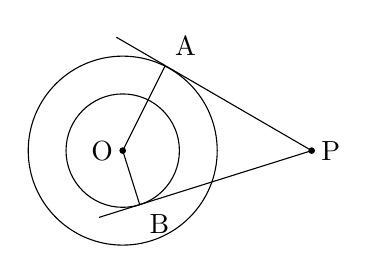
\begin{tikzpicture}[scale=1.2]
  % Draw the large circle
  \draw (0,0) circle (1cm);
  
  % Draw the middle circle
  \draw (0,0) circle (0.6cm);
  
  % Label the center
  \fill (0,0) circle (1pt) node[left] {O};
  
  % Draw the point P and line OP
  \fill (2,0) circle (1pt) node[right] {P};
  
  
  % Draw and label the tangent line
  \draw (2,0) -- (0.45,0.9) node[above right] {A};
  \draw (2,0) -- (0.18,-0.57148) node[below right] {B};
  
  % Optional: Add arrows to the line to indicate it extends indefinitely
  \draw (0.45,0.9) -- (-0.067,1.2);
  \draw (0.18,-0.57148) -- (-0.25,-0.7065);
  \draw (0,0) -- (0.45,0.9);
  \draw (0,0) -- (0.18,-0.57148);
  
\end{tikzpicture}
\end{figure}
\begin{center}
$\text{Figure } 12$
\end{center}

%circles
\item In Figure $13$, an isosceles triangle $ABC$, with $AB = AC$, circumscribe a circle. Prove that the point of contact $P$ bisects the base $BC$.
\begin{figure}[ht]
\centering
\begin{tikzpicture}[scale=0.3]
  % Define coordinates for the vertices of the triangle
  \coordinate[label=left:$B$] (B) at (0,0);
  \coordinate[label=right:$C$] (C) at (10,0);
  \coordinate[label=above:$A$] (A) at (5,8.6603);

  % Draw the triangle
  \draw (A) -- (B) -- (C) -- cycle;

 % Draw the circle with centre (0.5,0.28868) and radius 0.28868
    \draw (5,2.8868) circle (2.8868);

  % Label the incenter. Adjust the label position as needed
  \coordinate[label=left:$R$] (R) at (2.5,4.33015);
  \coordinate[label=above:$P$] (P) at (5,0);
  \coordinate[label=right:$Q$] (Q) at (7.5,4.33015);
  
  % Drawing perpendicular lines
  \draw ($(P)!0.1cm!90:(B)$) -- ($(P)!0.1cm!-90:(B)$);
  \draw ($(R)!0.1cm!90:(B)$) -- ($(R)!0.1cm!-90:(B)$);
  \draw ($(Q)!0.1cm!90:(C)$) -- ($(Q)!0.1cm!-90:(C)$);

\end{tikzpicture}
\end{figure}
\begin{center}
$\text{Figure } 13$
\end{center}
%circles
\item In Figure $14$, the chord $AB$ of the larger of the two concentric circles, with centre $O$, touches the smaller circle at $C$. Prove that $AC = CB$.
\begin{figure}[ht]
\centering
\begin{tikzpicture}[scale=1.5]
  \draw (0,0) circle (1cm);
  
  % Draw the middle circle
  \draw (0,0) circle (0.5cm);
  
  % Label the center
  \fill (0,0) circle (1pt) node[above] {O};
  
  % Draw the points P, A, B, and lines OP, AC, BC
  \coordinate[label=below:C] (C) at (0,-0.5);
  \coordinate[label=left:A] (A) at (-0.866,-0.5);
  \coordinate[label=right:B] (B) at (0.866,-0.5);
  
  % Draw and label the tangent line
  \draw (-0.866,-0.5) -- (0.866,-0.5);
  \draw ($(C)!0.1cm!90:(A)$) -- ($(C)!0.1cm!-90:(A)$);
\end{tikzpicture}
\end{figure}
\begin{center}
$\text{Figure } 14$
\end{center}
%circles
\item In Figure $15$, $OABC$ is a square of side $7 \text{ cm}$. If $OAPC$ is a quadrant of a circle with centre $O$, then find the area of the shaded region. $\brak{\text{Use } \pi = 3.14}$ 
 
\begin{figure}[ht]
\centering
\begin{tikzpicture}[scale=0.3]
    % Draw the square
    \draw[thick] (0,0) rectangle (7,7);
    
    % Add the hatching pattern with controlled density
    \path[pattern=north east lines, pattern color=black] (0,0) rectangle (7,7);
    
    % Draw the quadrants
    \draw[thick,fill=white] (0,0) -- (7,0) arc [start angle=0, end angle=90, radius=7] -- cycle;

    % Label the vertices
    \node at (0,0) [below left] {O};
    \node at (7,0) [below right] {A};
    \node at (7,7) [above right] {B};
    \node at (0,7) [above left] {C};
    \node at (5,5) [below left] {P};
    \fill (4.9,5) circle (2pt);

\end{tikzpicture}
\end{figure}
\begin{center}
$\text{Figure } 15$
\end{center}

\item Prove that the parallelogram circumscribing a circle is rhombus. 
%circles
\item Prove that opposite sides of a quadrilateral circumscribing a circle subtend supplementary angles at the centre of the circle. 
%circles
\item In Figure $16$, $PQ$ and $AB$ are respectively the arcs of two concentric circles of radii $7\text{ cm}$ and $3.5\text{ cm}$ and centre $O$. If $\angle POQ = 30\degree$, then find the area of the shaded region. $\brak{\text{Use } \pi = \frac{22}{7}}$
\begin{figure}[ht]
\centering
\begin{tikzpicture}[rotate = -20, scale = 0.48]

   \coordinate (O) at (0,0);
   \coordinate (A) at (2.7,2.25);
   \coordinate (B) at (3.5,0);
   \coordinate (P) at (5.4,4.5);
   \coordinate (Q) at (7,0);

    % Draw the quadrants
    \draw[thick] (0,0) -- (7,0) arc [start angle=0, end angle=40, radius=7] -- cycle;
    
    % Add the hatching pattern with controlled density
    \path[pattern=north west lines, pattern color=black] (0,0) -- (7,0) arc [start angle=0, end angle=40, radius=7] -- cycle;

    \draw[thick,fill=white] (0,0) -- (3.5,0) arc [start angle=0, end angle=40, radius=3.5] -- cycle;

    % Label the vertices
    \node at (0,0) [left] {O};
    \node at (2.7,2.25) [above] {A};
    \node at (3.5,0) [below] {B};
    \node at (7,0) [below] {Q};
    \node at (5.4,4.5) [above] {P};

    % Draw the angle arc % Draw the angle with label
  \pic [draw, "$30^O$", angle eccentricity=1.75, angle radius=0.6cm] {angle = Q--O--P};

\end{tikzpicture}
\end{figure}
\begin{center}
$\text{Figure } 16$
\end{center}
\item Prove that the tangent at any point of a circle is perpendicular to the radius through the point of contact. 

\item A quadrilateral $ABCD$ is drawn to circumscribe a circle. Prove that $AB + CD = AD + BC$. 

\item The incircle of an isosceles triangle $ABC$, with $AB = AC$, touches the sides $AB$, $BC$ and $CA$ at $D$, $E$ and $F$ respectively. Prove that $E$ bisects $BC$. 

\item Prove that in two concentric circles. the chord of the larger circle, which touches the smaller circle, is bisected at the point of contact. 

\item In Figure $17$, the shape of the top of the table is that of a sector of a circle with centre $O$ and $\angle OAB = 90\degree$. If $AO = OB = 42\text{ cm}$, then find the perimeter of the top of the table.
\begin{figure}[ht]
\centering
\begin{tikzpicture}[rotate = -45, scale = 1.5]

  % Define points for the angles
  \coordinate (O) at (0,0);
  \coordinate (A) at (0,-1);
  \coordinate (B) at (1,0);

  % Right angle at B
  \draw pic["$ $", draw=black, angle radius=0.35cm, angle eccentricity=1.5] {right angle = A--O--B};
  
  % Draw the sectors and lines
  \draw (O) -- (A) (O) -- (B);

  % Draw the quadrants
  \draw[fill=white] (O) -- (B) arc [start angle=0, end angle=270, radius=1] -- cycle;
  
  % Label the center
  \node at (O) [above] {O};
  \node at (A) [below left] {A};
  \node at (B) [below right] {B};

\end{tikzpicture}
\end{figure}
\begin{center}
$\text{Figure } 17$
\end{center}
\item Find the area of the shaded region in Figure $18$, if $ABCD$ is a square of side $28\text{ cm}$ and $APD$ and $BPC$ are semicircles.
\begin{figure}[ht]
\centering
\begin{tikzpicture}[scale=0.6]
  % Draw square
  \draw (0,0) rectangle (4,4);
  
  % Label corners of the square
  \coordinate (O) at (2,4.2);
  \node at (-0.2,-0.2) {A};
  \node at (4.2,-0.2) {B};
  \node at (4.2,4.2) {C};
  \node at (-0.2,4.2) {D};
  \coordinate (P) at (2,2);
  \node at (2,2) [left] {P};
  
  % Draw and fill the area between the arcs
  \begin{scope}
    \clip (0,4) arc[start angle=90, end angle=-90, radius=2] -- 
          (4,0) arc[start angle=-90, end angle=-270, radius=2];
    \fill[pattern=north east lines] (0,0) rectangle (4,4);
  \end{scope}

  % Drawing perpendicular lines
  \draw ($(P)!0.1cm!90:(O)$) -- ($(P)!0.1cm!-90:(O)$);
  
  % Draw arcs again on top of the fill to make them visible
  \draw (0,4) arc[start angle=90, end angle=-90, radius=2];
  \draw (4,0) arc[start angle=-90, end angle=-270, radius=2];

\end{tikzpicture}
\end{figure}
\begin{center}
$\text{Figure } 18$
\end{center}
\item Two tangents $TP$ and $TQ$ are drawn to a circle with centre $O$ from an external point $T$. Prove that $\angle TPQ = 2\angle OPQ$. 

\item In Figure $19$, $XY$ and $X'Y'$ are two parallel tangents to a circle with centre $O$ and another tangent $AB$ with point of contact $C$ intersects $XY$ at $A$ and $X'Y'$ at $B$. Prove that $\angle AOB = 90\degree$
\begin{figure}[ht]
\centering
\begin{tikzpicture}[scale = 0.3]

  % Draw the circle
  \draw (0,0) circle (5cm);
  
  % Define points for the angles
  \coordinate (O) at (0,0);
  \coordinate (A) at (7.2,5);
  \coordinate (B) at (3.5,-5);
  \coordinate (C) at (4.55,-2);
  \coordinate (P) at (0,5);
  \coordinate (Q) at (0,-5);
  \coordinate (X) at (-7.5,5);
  \coordinate (Y) at (7.5,5);
  \coordinate (X') at (-7.5,-5);
  \coordinate (Y') at (7.5,-5);

  % Draw the sectors and lines
  \draw (O) -- (A) (O) -- (B) (A) -- (B);
  \draw (P) -- (X) (P) -- (Y) (Q) -- (X') (Q) -- (Y');
  \draw (O) -- (P) (O) -- (Q);

  % Arrows
  \draw[->] (P) -- ($(P)!8.5cm!(X)$);
  \draw[->] (P) -- ($(P)!8.5cm!(Y)$);
  \draw[->] (Q) -- ($(Q)!8.5cm!(X')$);
  \draw[->] (Q) -- ($(Q)!8.5cm!(Y')$);
  
  % Label the center
  \node at (O) [left] {O};
  \node at (A) [above] {A};
  \node at (B) [below] {B};
  \node at (C) [right] {C};
  \node at (P) [above] {P};
  \node at (Q) [below] {Q};
  \node at (X) [above] {X};
  \fill (X) circle (2pt);
  \node at (Y) [above] {Y};
  \fill (Y) circle (2pt);
  \node at (X') [below] {X'};
  \fill (X') circle (2pt);
  \node at (Y') [below] {Y'};
  \fill (Y') circle (2pt);

\end{tikzpicture}
\end{figure}
\begin{center}
$\text{Figure } 19$
\end{center}
\item In Figure $20$, $ABCD$ is a square of side $7\text{ cm}$. $DBPA$ and $DQBC$ are quadrants of circles, each of radius $7\text{ cm}$. Find the area of the shaded region.$\brak{\text{Use } \pi = \frac{22}{7}}$
\begin{figure}[ht]
\centering
\begin{tikzpicture}[scale=0.5]
    % Draw the square
    \draw (0,0) rectangle (7,7);
    
    % Draw the arcs
    \draw (0,0) -- (7,0) arc [start angle=0, end angle=90, radius=7] -- cycle;
    \draw (7,7) -- (0,7) arc [start angle=180, end angle=270, radius=7] -- cycle;

    % Shade the region between the arcs
    \begin{scope}
        \clip (0,0) -- (7,0) arc [start angle=0, end angle=90, radius=7] -- cycle;
        \fill[pattern=north east lines, pattern color=black] (7,7) -- (0,7) arc [start angle=180, end angle=270, radius=7] -- cycle;
    \end{scope}

    % Label the vertices
    \node at (0,0) [below left] {A};
    \node at (7,0) [below right] {B};
    \node at (7,7) [above right] {C};
    \node at (0,7) [above left] {D};
    \node at (4.9,5) [above right] {P};
    \node at (2.05,2.05) [below left] {Q};
    \fill (4.9,5) circle (1pt);
    \fill (2.05,2.05) circle (1pt);

\end{tikzpicture}
\end{figure}
\begin{center}
$\text{Figure } 20$
\end{center}
\item The length of the minute hand of a clock is $14\text{ cm}$. Find the area swept by the minute hand in $10$ minutes. $\brak{\text{Use } \pi = \frac{22}{7}}$ 
\item Prove that the tangent at any point of a circle is perpendicular to the radius through the point of contact. 
\end{enumerate}
